\documentclass[a4paper, 12pt]{article}
\usepackage[utf8]{inputenc}
\usepackage{listings}
\usepackage{graphicx}
\usepackage{natbib}

\title{Requirement specification}
\author{Logistics administration for Transport AS}
\date{April 2020}

\begin{document}
\maketitle

\section{Introduction}
\subsection{Purpose}
Transport AS is a company that handles home delivery missions from a local storage. The purpose of this software is to help the logistics administrator to manage deliveries and for transport workers to get information about their missions.
\subsection{Limitations}
In this project functionality is prioritised over security.
User authentication is disregarded because of project timeconstraints.

\subsection{Users}
\begin{itemize}
     \item Logistics administrator
     \item Transport worker
\end{itemize}
\subsection{Overview}
An administrator would add a transportation worker, transportation vehicle. The administrator would then create a new mission with a transportation worker and a transportation vehicle. The transportation worker would then view the transportation missions to see his work for the coming time. A transportation worker would then mark the mission as completed when he completes the mission. Only the logistics administrator would be able to mark missions as canceled.
 \begin{figure}[h]
    \centering 
    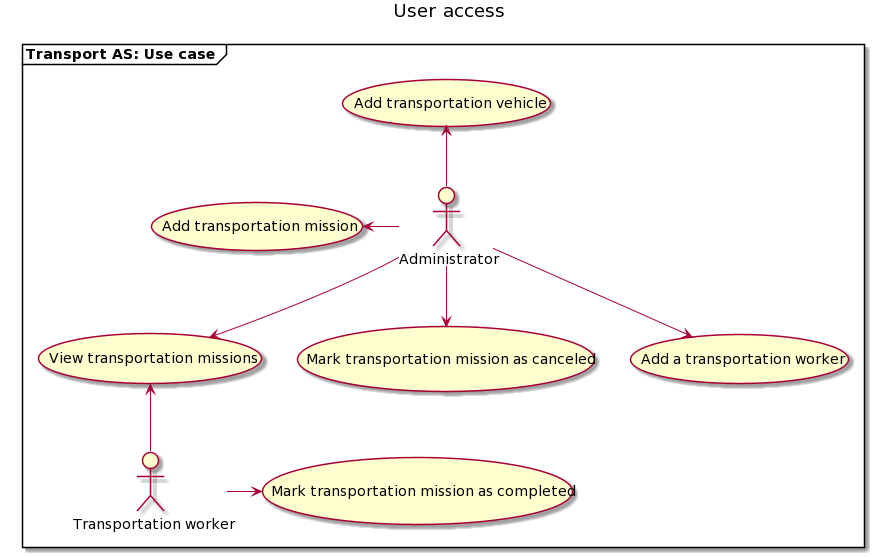
\includegraphics[width=0.7\textwidth]
    {img/user-access-uc}
    \caption{User-access use case}
    \label{fig:ua-uc}
  \end{figure}
  
\section{Requirements}
\subsection{Functional requirements}
\begin{itemize}
  \item F 1.0 Logistics administrator shall be able to add new transportation vehicles
  \item F 1.1 Logistics administrator shall be able to add new transportation missions
  \item F 1.2 Logistics administrator shall be able to add transportation vehicles to transportation missions
  \item F 1.3 Logistics administrator shall be able to mark transportation mission as canceled
  \item F 1.4 Logistics administrator shall be able to add a transportation worker
  \item F 1.5 Logistics administrator shall be able to add a transportation to a vehicle
  \item F 1.6 Transport worker shall be able to view transportation missions
  \item F 1.7 Transport worker shall be able to mark transportation missions as completed
\end{itemize}
\subsection{Non-functional requirments}
\begin{itemize}
  \item N 1.0 Database shall be hosted in Azure SQL Database
  \item N 2.0 Website shall be written in HTML5
  \item N 2.1 Website shall use CSS for styling
  \item N 3.0 Web-application shall use Flask web-framework
  \item N 3.1 Web-application shall use SQL-Alchemy as an ORM
\end{itemize}

\section{Time estimation}
T-shirt sizing:
\begin{itemize}
\item Large
\item Medium
  \item Small
\end{itemize}
\begin{center}
\begin{tabular}{ |c|c|c| } 
  \hline
  \multicolumn{2}{|c|}{Time estimation of requirements} \\
  \hline
  F 1.0 & Medium \\
  \hline
  F 1.1 & Medium \\
  \hline
  F 1.2 & Medium \\
  \hline
  F 1.3 & Small \\
  \hline
  F 1.4 & Small \\
  \hline
  F 1.5 & Medium \\
  \hline
  F 1.6 & small \\
  \hline
  F 1.7 & Medium \\
 \hline
\end{tabular}
\end{center}
\end{document}
%%% Local Variables:
%%% mode: latex
%%% TeX-master: t
%%% End:
